\documentclass{beamer}

\usepackage{amsthm}
\usepackage[utf8]{inputenc}
\usepackage[T1]{fontenc}
\usepackage[brazil]{babel}
\usepackage[export]{adjustbox}
\usepackage{listings}
\usepackage{fontspec}
\usepackage{color}

\definecolor{pblue}{rgb}{0.13,0.13,1}
\definecolor{pgreen}{rgb}{0,0.5,0}
\definecolor{pred}{rgb}{0.9,0,0}
\definecolor{pgrey}{rgb}{0.46,0.45,0.48}

\lstset{language=Java,
  showspaces=false,
  showtabs=false,
  breaklines=true,
  showstringspaces=false,
  breakatwhitespace=true,
  commentstyle=\color{pgreen},
  keywordstyle=\color{pblue},
  stringstyle=\color{pred},
  basicstyle=\ttfamily,
}


\usetheme{Madrid}
\usecolortheme{beetle}
\usefonttheme{professionalfonts}

\setmainfont{Oswald}

\lstset{basicstyle=\ttfamily,breaklines=true}
\beamertemplatenavigationsymbolsempty

\begin{document}

\selectlanguage{brazil}
\title[Complexidade]{Complexidade de Algoritmos}
\author{Prof. Andrey Masiero}

\begin{frame}[plain,noframenumbering]
  \titlepage
\end{frame}

\begin{frame}[plain,noframenumbering]
  \frametitle{Agenda}
  \tableofcontents
\end{frame}

\section{Introdução}

\begin{frame}
	\frametitle{Introdução}
    \begin{itemize}[<+->]
        \item Identificar se a complexidade do problema e algoritmo proposto, geram uma solução eficiente ou não;
        \item Técnicas de programação auxiliam durante a implementação dele (Estrutura de Dados, Métodos de Divisão de Problema, etc);
        \item A análise é feita a partir de uma entrada $n$ de elementos, como é o comportamento do algoritmo.
    \end{itemize}
\end{frame}

\begin{frame}
	\frametitle{Introdução}
    Como é feita a análise?
    \begin{itemize}[<+->]
        \item Remover elemento de um vetor com $n$ elementos: \\ No pior caso, leva $n-1$ iterações;
        \item Alterar elemento na posição $i$ do vetor: \\ Leva $1$ iteração;
        \item E assim por diante.
    \end{itemize}
\end{frame}

\section{Exemplos}

\begin{frame}
	\frametitle{Exemplo 01}
    Determinar quantas vezes o laço executa:
    \lstinputlisting[language=Java]{src/exemplo1.java}
\end{frame}

\begin{frame}
	\frametitle{Exemplo 02}
    E esse outro laço, quantas vezes executa:
    \lstinputlisting[language=Java]{src/exemplo2.java}
\end{frame}

\begin{frame}
	\frametitle{Analisando os exemplos 01 e 02}
    \begin{itemize}[<+->]
        \item Número de repetições do exemplo 1 = 1000;
        \item Número de repetições do exemplo 2 = n;
        \item Então pode-se dizer que o número de repetições é de acordo com $n$;
        \item Sendo assim, minha função é $f(n) = n$.
    \end{itemize}
\end{frame}

\begin{frame}
	\frametitle{Exemplo 03}
    \lstinputlisting[language=Java]{src/exemplo3.java}
\end{frame}

\begin{frame}
	\frametitle{Exemplo 04}
    \lstinputlisting[language=Java]{src/exemplo4.java}
\end{frame}

\begin{frame}
	\frametitle{Analisando os exemplos 03 e 04}
    \begin{itemize}[<+->]
        \item Se observarmos a operação $i \times 2$, é a mesma coisa que $2^i$;
        \item Sendo assim, o exemplo 3 tem 10 repetições;
        \item Número de repetições do exemplo 4 = ?;
        \item Na matemática, para esse caso, o $n$ é encontrado por uma função $\log_2$;
        \item Então, o número de repetições do exemplo 4 = $\log_2 n$;
        \item Pode-se dizer que o número de repetições é de acordo com $\log_2 n$;
        \item Minha função resulta em $f(n) = \log_2 n$.
    \end{itemize}
\end{frame}

\begin{frame}
	\frametitle{Exemplo 05}
    \lstinputlisting[language=Java]{src/exemplo5.java}
\end{frame}

\begin{frame}
	\frametitle{Analisando os exemplos 05}
    \begin{itemize}[<+->]
        \item Analisando o primeiro \texttt{for} ele tem o número de repetições = $n$;
        \item O segundo \texttt{for} ele tem o número de repetições = $\log_2 n$;
        \item Combinando os dois temos $n \times \log_2 n$;
        \item Minha função fica: $f(n) = n\log_2 n$.
    \end{itemize}
\end{frame}

\begin{frame}
	\frametitle{Exemplo 06}
    \lstinputlisting[language=Java]{src/exemplo6.java}
\end{frame}

\begin{frame}
	\frametitle{Analisando os exemplos 06}
    \begin{itemize}[<+->]
        \item Analisando o primeiro \texttt{for} ele tem o número de repetições = $n$;
        \item O segundo \texttt{for} ele tem o número de repetições = $n$;
        \item Combinando os dois temos $n \times n$;
        \item Minha função fica: $f(n) = n^2$.
    \end{itemize}
\end{frame}

\section{Notação Big O}

\begin{frame}
	\frametitle{Notação Big O}
    \begin{itemize}
        \item Em complexidade de algoritmos utilizamos a notação $O(f(n))$ para dizer qual é o tempo de execução do algoritmo, no pior caso;
        \item Então se minha função é $f(n) = n^2$;
        \item Na notação Big O é: $O(n^2)$.
    \end{itemize}
\end{frame}

\section{Categoria de Grandezas}

\begin{frame}
	\frametitle{Categoria de Grandezas}
    \begin{itemize}
        \item Logarítmica: $\log_2 n$;
        \item Linear: $n$;
        \item Logarítmica Linear: $n\log_2 n$;
        \item Quadrática: $n^2$;
        \item Polinomial: $n^k$;
        \item Exponencial: $2^n$;
        \item Fatorial: $n!$.
    \end{itemize}
\end{frame}

\begin{frame}
    \frametitle{Categoria de Grandezas}
    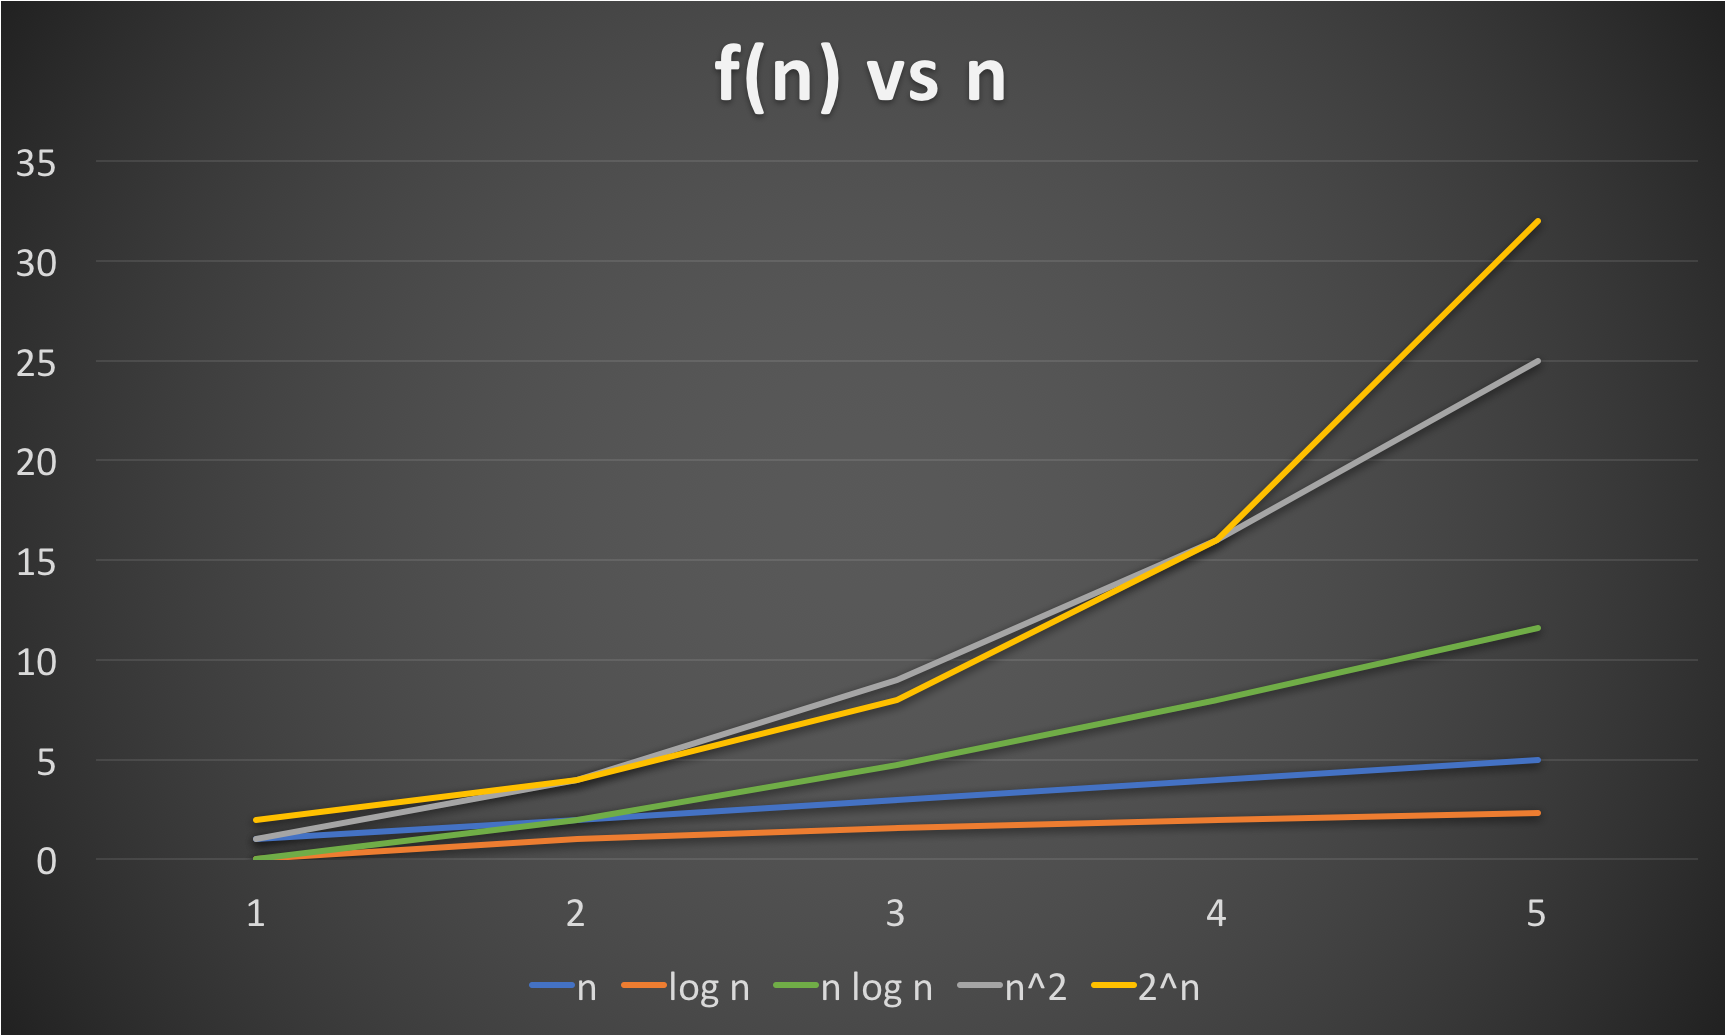
\includegraphics[width=\textwidth]{images/grafico_funcoes.png}
\end{frame}


\section{Exercícios}

\begin{frame}
    \frametitle{Exercícios}
    \begin{itemize}
        \item Analise os códigos a seguir e encontre sua complexidade.
        \item Diga a complexidade na notação Big O.
    \end{itemize}
\end{frame}

\begin{frame}
	\frametitle{Exercício 01}
    \lstinputlisting[language=Java]{src/exercicio1.java}
\end{frame}

\begin{frame}
	\frametitle{Exercício 02}
    \lstinputlisting[language=Java]{src/exercicio2.java}
\end{frame}

\begin{frame}
	\frametitle{Exercício 03}
    \lstinputlisting[language=Java]{src/exercicio3.java}
\end{frame}

\section{Referências}

\begin{frame}
    \frametitle{Referências Bibliográficas}
    \begin{enumerate}
        \item Cormen, Thomas H., Charles E. Leiserson, Ronald L. Rivest, and Clifford Stein. ``Introduction to algorithms second edition.'' (2001).
        \item Tamassia, Roberto, and Michael T. Goodrich. ``Estrutura de Dados e Algoritmos em Java.'' Porto Alegre, Ed. Bookman 4 (2007).
        \item Ascencio, Ana Fernanda Gomes, and Graziela Santos de Araújo. ``Estruturas de Dados: algoritmos, análise da complexidade e implementações em JAVA e C/C++.'' São Paulo: Perarson Prentice Halt 3 (2010).
    \end{enumerate}
\end{frame}

\end{document}
